%!TEX root = ../Main.tex

\chapter{Design}
\section{Design Patterns}
\subsection{State Machine Pattern}
The state machine pattern has been used to develop the system. This is partly in order to structure the general flow of the algorithm, and partly in order to support concurrent development of the algorithm, as different parts of the algorithm can be implemented simultaneously as different states.

Figure \ref{fig:STM_diagram} shows the state machine diagram for system. It can be seen that the general flow of the system is as follows:
\begin{enumerate}
	\item Set up system.
	\item Create initial population.
	\item Evaluate generation.
	\item If stopping criterion is met, save population and stop. Else-  create new generation, then return to step 3.
\end{enumerate}

\begin{figure}[H]
	\centering
	{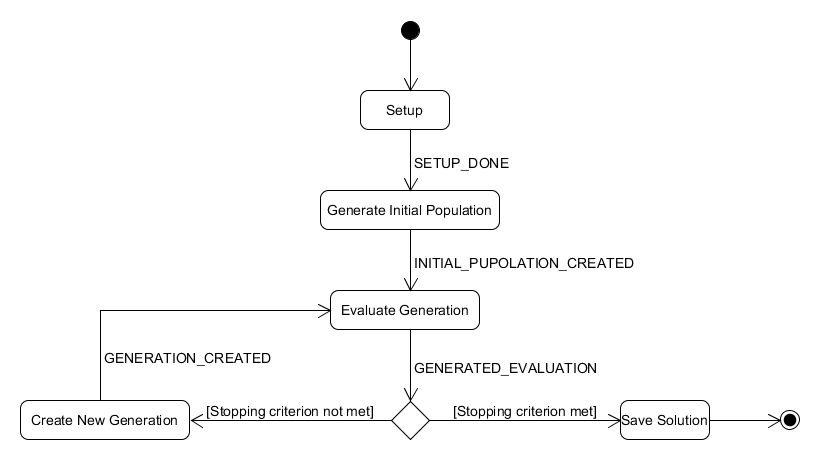
\includegraphics[width=\textwidth]{Images/STM_ROGSAnne.PNG}}\\[0.5cm]
	\caption{State machine diagram for the developed system.}
	\label{fig:STM_diagram}
\end{figure}

\subsection{Double buffering}
The implemented algorithm operates with two buffers, one for the new generation and one for the old generation. This means when a new generation is generated the memory is allocated for the new generation beforehand. The memory for the new generation could also have been allocated dynamically which would require less memory. But, by allocating the memory beforehand makes it possible to parallelize the process of generating a new generation in the future.

State pattern is the only software design pattern implemented in the system. The idea was also to implement the Command pattern, but because only one part of the system is getting hardware accelerated, it seemed a bit exaggerated to implement the Command pattern as well. The Command pattern could be used for the creation of a new generation, by creating a command queue and letting different instances of the class that creates samples \textit{(creators)} execute the commands, it is possible to "order" the creation of a certain amount of new samples, and then let the execution be up to the scheduler. This way, design space exploration can be carried out, with evaluation of execution speed versus resources used.

